%% grundlagen.tex
%% $Id: grundlagen.tex 28 2007-01-18 16:31:32Z bless $
%%

\chapter{Grundlagen}
\label{ch:Grundlagen}
%% ==============================
Die Grundlagen müssen soweit beschrieben
werden, dass ein Leser das Problem und
die Problemlösung  versteht.Um nicht zuviel 
zu beschreiben, kann man das auch erst gegen 
Ende der Arbeit schreiben.

Bla fasel\ldots

%% ==============================
\section{Persönlichkeitspsychologie}
%% ==============================
\label{ch:Grundlagen:sec:Abschnitt1}

Zentral für diese Arbeit ist die Geselligkeit eines Menschen.
Wissenschaftlich fällt das Betrachten dieser Persönlichkeitseigenschaft in den Bereich der Persönlichkeitspsychologie,
oft auch Differenzielle Psychologie genannt. 
Dieser Zweig der Pychologie beschäftigt sich mit den Unterschieden zwischen verschiedenen Personen, 
basierend auf Funktionen, Fähigkeiten und Verhalten, deren Ursprünge und der Konsequenzen der selben.
Sie bildet eine Grundlage für praktische Anwendung unter anderem im klinischen oder pädagogischen Kontext.
\par

Historisch begonnen hat das Fachgebiet mit der Intelligenzforschung und Quantifizierung, 
die auch Heute noch ein wichtiger Grundpfeiler der Differenziellen Psychologie ist.
Im Laufe der Zeit kamen weitere Thematiken hinzu wie Temperatmenteigenschaften, Einstellungen und, für diese Arbeit relevant, Sozialverhalten.
\par

Bisher konnte sich keine allgemeine, allumfassende Persönlichkeitstheorie durchsetzten, sondern es gibt eine breite Masse an verschiedenen Ansätzen und Menschenbildern, die von verschiedenen Theoretikern unterstützt werden
\ignore{ Beispiel Sigmund Freund?}
Im Rahmen dieser Arbeit wird mit dem "`Big Five"' Persönlichkeitsmodell gearbeitet, das im deutschsprachigen Raum auch manchmal das "`Fünf Faktoren Modell"' genannt wird.
Es ist, neben dem Myers-Briggs Type Indicator, eines der bekanntesten, meistgenutzten Modelle und wird der Forschung weithin anerkannt.
Das Big Five Modell bietet sich speziell für diese Arbeit an, da es bei diesem Modell sehr einfach ist, nur den Geselligkeits Aspekt und direkt zusammenhängende Aspekte zu betrachten.

\subsection{Big Five Modell}

Nach dem Big Five Modell existieren fünf Hauptdimensionen, die die Grundlage für die Persönlichkeit eines Menschen bilden.
Jeder Mensch lässt sich demnach auf 5 Skalen einordnen, wie sehr die folgendende Eigenschaften bei ihr ausgeprägt sind.

\begin{itemize}
  \item Openness to Experience (Offenheit für Erfahrungen)
  \item Neuroticism (Neurotizismus)
  \item Conscientiousness (Gewissenhaftigkeit)
  \item Agreeableness (Verträglichkeit)
  \item Extraversion
\end{itemize}

Das Big Five Modell verfolgt hierbei einen lexikalischen Ansatz: 
Persönlichkeitsmerkmale schlagen sich in der Sprache der sprechenden Person nieder.
Eine Faktorenanalyse über eine Liste von 18.000 Begriffen ergab die fünf oben stehenden Faktoren.
Diese bleiben über die Lebensspanne stabil und können in den verschiedensten Kulturen beobachtet werden.

\subsection{NEO-PI-R}

Der "`NEO - Personality Inventory - Revised"' ist ein Persönlichkeitstest, der das Big Five Modell implementiert.
Der NEO-PI-R ist eine 1990 erstmals veröffentlichte überarbeitete Version des NEO-Pi's von 1978 und hat seitdem mehrere Aktualisierungen bekommen. Die aktuellste Version ist von 2010.
Basierend auf 241 Aussagen, zu denen die Probandin mit 5 Abstufungen von "`Starke Ablehnung"' bis "`Starke Zustimmung"' ihre Meinung darlegt, legt der Test die 5 Hauptfaktoren plus jeweils 6 Unterfacetten dar.
Die 6 Facetten des für diese Arbeit relevanten Extraversion Faktors sind:

\begin{itemize}
  \item Warmth (Herzlichkeit)
  \item Gregariousness (Geselligkeit)
  \item Assertiveness (Durchsetzungsfähigkeit)
  \item Activity (Aktivität)
  \item Excitement-Seeking (Erlebnishunger)
  \item Positive Emotions (Frohsinn)
\end{itemize}

Im Rahmen dieser Arbeit soll der Fokus vorallem auf der Geselligkeitsfacette liegen.

%% ==============================
\section{Smartphones}

\label{ch:Grundlagen:sec:Abschnitt2}


Als Smartphone wird allgemeinhin ein Mobiltelefon bezeichnet, das zusätzlich zu den herkömmlichten Funktionalitäten eines Mobiltelefons wie Anrufe und SMS Versand über verschiedene Features eines Personal Computers verfügt. 
Ausschlaggebend für die Klassifikation ist unteranderem das Vorhandensein eines mobilen Betriebssystems.
Typische Smartphonefeatures sind Internetfähigkeit, Touchscreen und die Möglichkeit ohne große Umstände Zusatzprogramme von Drittherstellern zu installieren.
Diese Zusatzprogramme werden im weiteren als Applikationen, oder kurz Apps, bezeichnet.
\par

Smartphones und mit ihnen das Mobile Web sind inzwischen ein wichtiger Faktor geworden:
2015 besaßen 80\% der Internet Nutzer zwischen 16 und 64 ein Smartphone. 
Damit ist das Smartphone das zweitrelevanteste Zugangsgerät hinter dem Desktop Computer, der mit 91\% an der Spitze steht. \cite{globalwebindex}
\par

Es gibt eine Vielzahl an verschiedenen Betriebsystemen mit einen Smartphone ausgestattet sein kann.
Jedoch ist der aktuelle Stand, dass der Markt von nur zwei Firmen dominiert wird.
Google's Android Betriebssystem, das mit 80.7\% Marktanteil von neu abgesetzten Geräten dominant an der Spitze steht
und Apple's IOs, das mit 17.7\% noch knapp mehr als ein sechstel der Smartphone Verkäufe aufzuweisen hat.
Dahinter liegen auf den Plätzen drei und vier Microsoft's Windows und Blackberry mit 1.1\% und 0.2\%\cite{smartphonemarktanteil}.
Dementsprechend wird sich dieser Arbeit Android als Standart angenommen.

\ignore{todo: insert pdf graphic}
\begin{figure}[h]
    \centering
    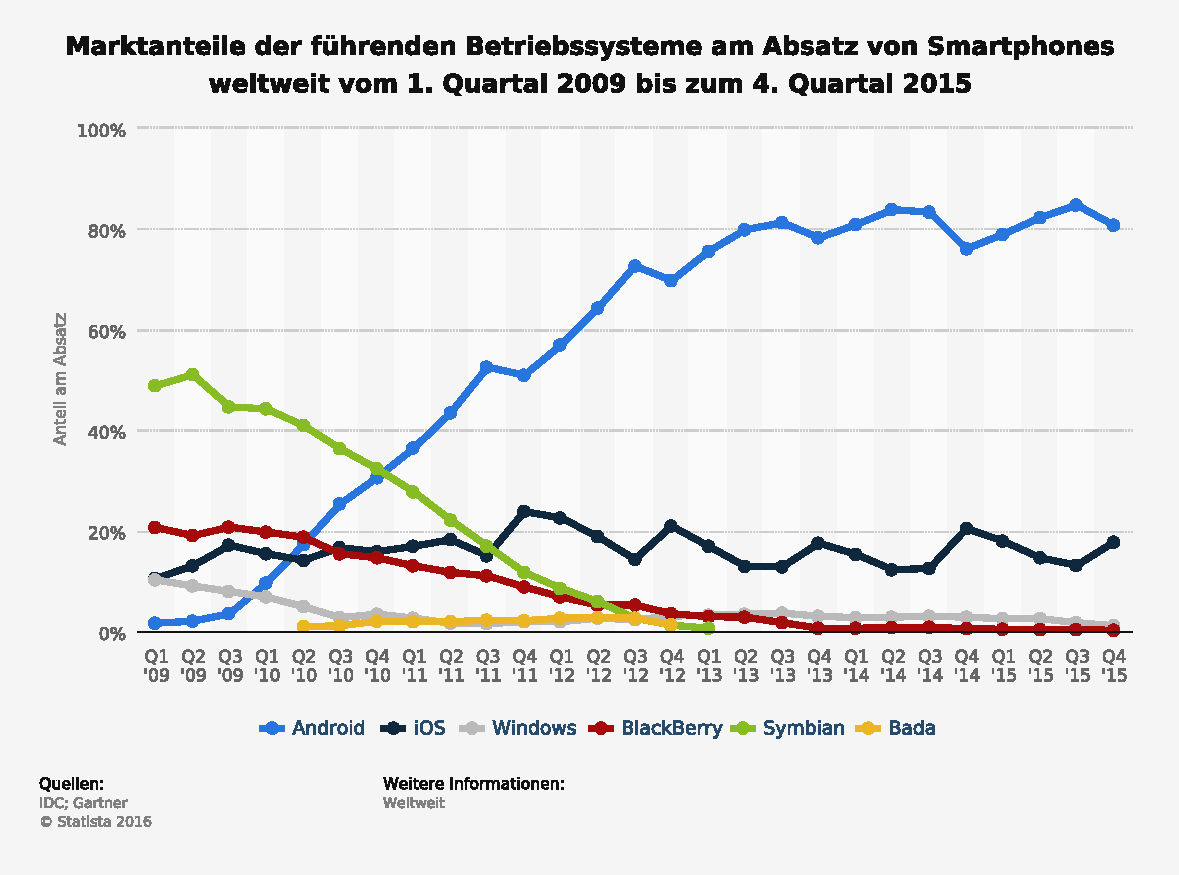
\includegraphics[width=\textwidth]{images/statistic_id73662_marktanteile-der-smartphone-betriebssysteme-am-absatz-weltweit-bis-q4-2015.pdf}
    \caption{Marktanteile der Smartphone Betriebssysteme am Absatz weltweit}
    \label{fig:marktanteil}
\end{figure}


\subsection {Android NotificationManager}

Notifications sind die vom Android Betriebssystem vorgesehene Art und Weise, 
wie eine Applikation die Nutzerin über einen Vorfall aufmerksam macht, während die Applikation nicht im Vordergrund ist.
Dies kann zum Beispiel im Falle der Signal Messenger App eine eingetroffene SMS sein,
oder der erfolgreiche Abschluss eines Updates vom Google Play Store.
Eine gepostete Notification taucht im Allgemeinen zunächst als kleines Pop-up am oberen Bildschirmrand auf und wird dann in die 
Notification Area (siehe \ref{fig:notificationarea}) abgelegt.
Durch das Öffnen des Notification Drawers (siehe \ref{fig:notificationdrawer}) kann eine detailiertere Ansicht aller ungelesenen Notifications geöffnet werden und gelesene beziehungsweise nicht relevante Notifications entfernt werden 
\cite{androidnotification}.
Die Nutzerin kann einstellen, welche Apps Notifications senden dürfen und welche nicht.
So wird ein Spiel, dass konstant auf sich selbst aufmerksam zu machen versucht wahrscheinlich geblockt,
während dem E-mail Client, der die Nutzerin auf neu angekommene E-mails aufmerksam macht, diese Berechtigung erteilt.
Dementsprechend ist anzunehmen, dass die tatsächlich erhaltenen Notifications die Interessen der Nutzerin wiederspiegeln.
\par

Der NotificationManager ist die Stelle im Android Betriebssystem mit denen Applikationen Zugriff auf alle Notifications bekommen und mit ihnen interagieren können.
Das beinhaltet beliebige Notifications zu erstellen oder gepostete Notifications zu löschen.
An den NotificationManager gebunden werden, kann ein sogenannter NotificationListener, mit die Applikation alle an den NotificationManager geschickten Notifications lesen kann.
Dies beinhaltet unter anderem
\begin{itemize}
    \item {Package} Applikation, die die Notification gepostet hat
    \item {Notification Titel} Titel, oft der Absender der Nachricht
    \item {ticker} Zusammenfassung der Notification für accessibility services
    \item {text} Inhalt der Notification
\end{itemize}
Dies ist eine potenziell leicht zu missbrauchende und falls missbraucht potenziell katastrophale Berechtigung, weshalb die Berechtigung nicht bei der Installation gegeben werden kann, sondern von Hand von der Nutzerin bestätigt werden muss. 

\begin{figure}[h]
    \centering
    
\includegraphics{images/notification_area.png}
    \caption{Notification Area\cite{androidnotification}}
    \label{fig:notificationarea}
\end{figure}

\begin{figure}[h]
    \centering
    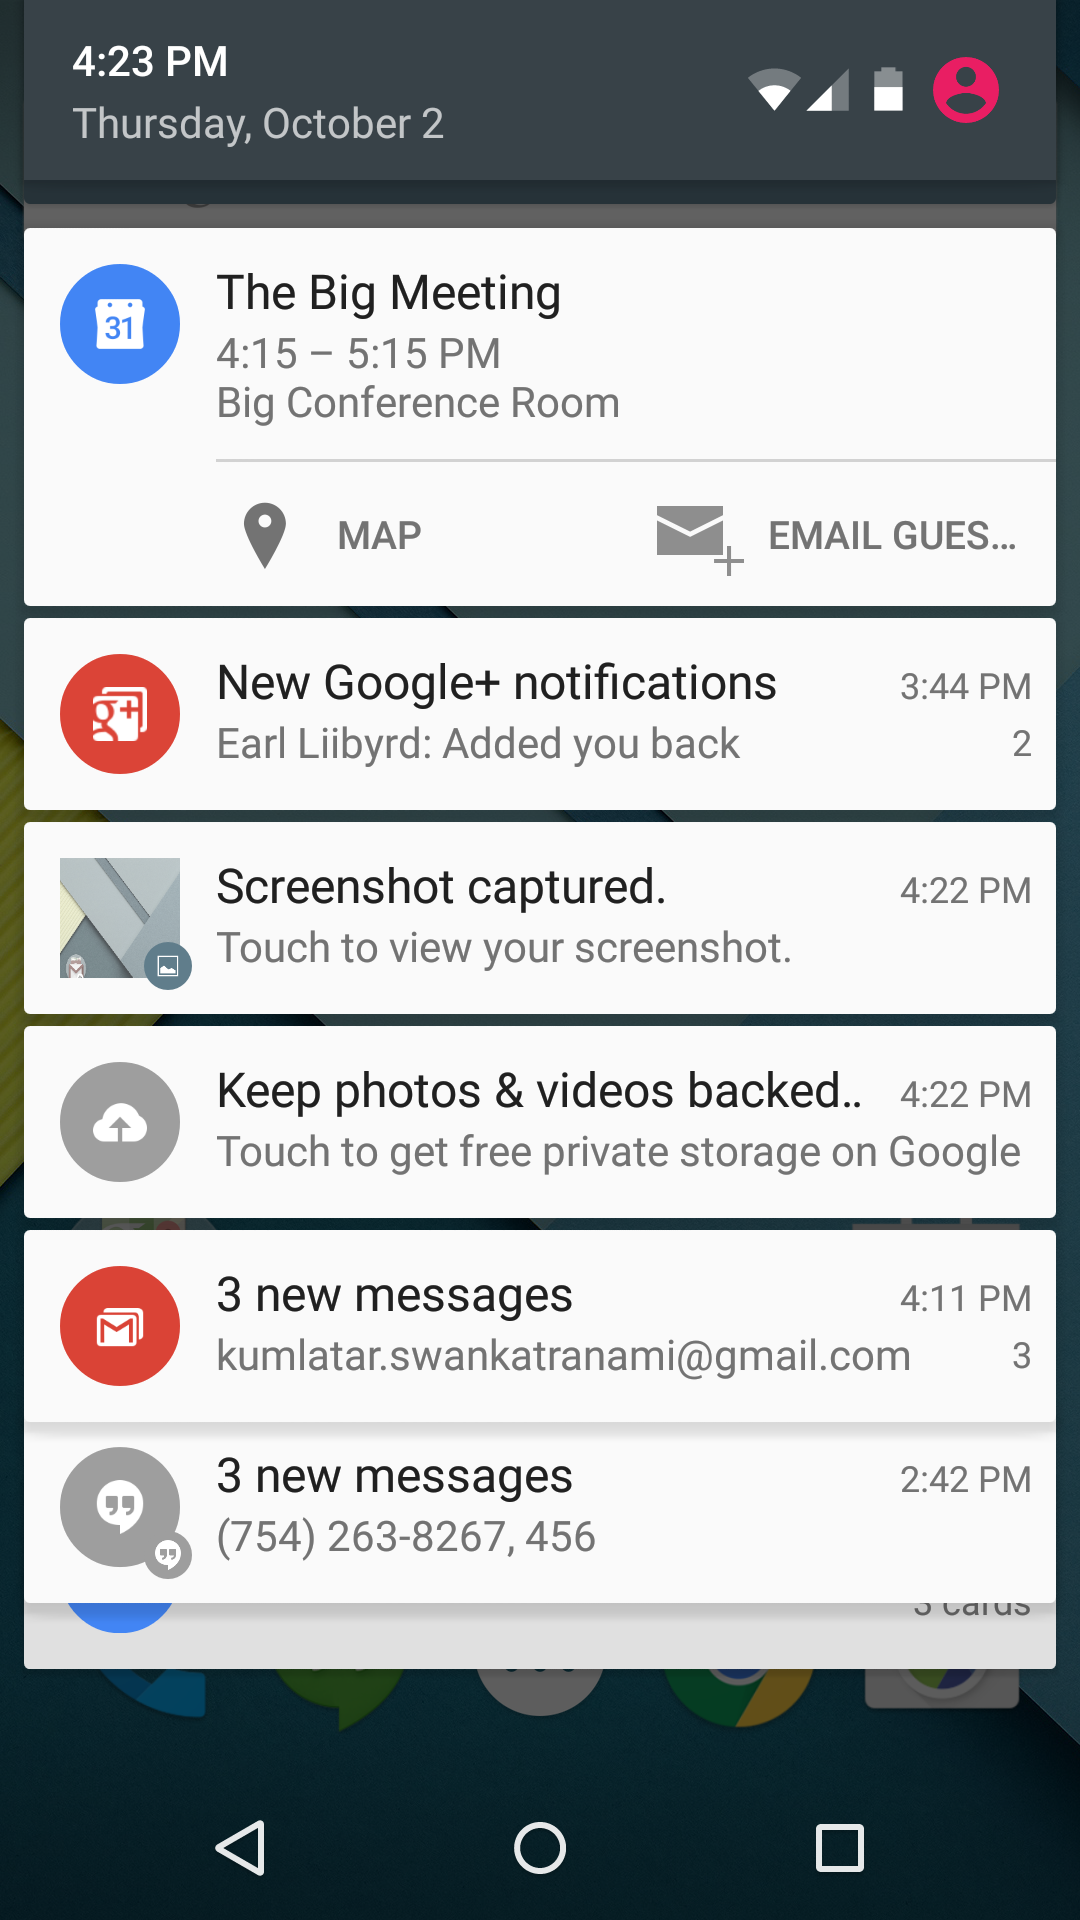
\includegraphics[width=0.5\textwidth]{images/notification_drawer.png}
    \caption{Notification Drawer\cite{androidnotification}}
    \label{fig:notificationdrawer}
\end{figure}



\subsection {Android UsageStatManager}

Der UsageStatManager ist eine Schnittstelle, die Zugang zu vom Betriebssystem gesammelten Daten
und Statistiken bezüglich der Nutzungshistorie des Geräts gibt \cite{androidusagestat}.
Die Methode \textbf{queryUsageStats(int intervalType, long beginTime, long endTime)} gibt eine Liste an UsageStats der verschiedenen Applikationen zurück.
Für jedes Element der Liste erhält man mit der Methode \textbf{getTotalTimeInForeground ()} die Zeit in Millisekunden,
die die App mit dem Package Namen aus \textbf{getPackageName ()} im Vordergrund war.
\par
Die UsageStatManager API benötigt die \textbf{android.permission.PACKAGE\_USAGE\_STATS} Permission.
Diese ist ebenfalls eine priviligierte Berechtigung, die Applikationen zwar beantragen können, die aber nicht bei der Installation erteilt werden kann, sondern nur von der Nutzerin von Hand beantragt werden kann.


%% ==============================
\section{Verwandte Arbeiten}
%% ==============================
\label{ch:Grundlagen:sec:RelatedWork}

Die steigende Relevanz von sowohl Smartphones als auch Social Media im alltäglichen Leben von vielen Menschen
motiviert eine Vielzahl an Studien und Papern sowohl zu jeweils den beiden Themen als auch der Überschneidung. 
\ignore{todo: hier sollte noch ein satz rein...}

In diesem Kapitel sollen einige Arbeiten betrachtet werden, die sich thematisch in der Nähe von dieser Arbeit befinden.



%%% Local Variables: 
%%% mode: latex
%%% TeX-master: "diplarb"
%%% End: 
